
\section{Problem Formulation and Existing Results}\label{sec:game-model}

In this section we first introduce the capacitated selfish replication game with binary preferences as was introduced in \cite{gopalakrishnan2012cache}. In the balance of this paper, our focus will be on such games, which for simplicity we refer to as CSR games.

\subsection{CSR Game Model}
We start with a set of $[n]=\{1,2,\ldots,n\}$ nodes (players) which are connected by an undirected graph $\mathcal{G}=([n], \mathcal{E})$. We denote the set of all resources by $O=\{o_1, o_2,\ldots, o_k\}$. For simplicity, but without much loss of generality, we assume that each node can hold only one resource in its cache. All the results can in fact be extended to CSR games with different capacities (see Remark \ref{rem:varying-cache} below). Moreover, we assume that each node has access to all the resources. For a particular allocation $P=(P_1, P_2, \ldots, P_n)$, we define the sum cost function $C_i(P)$ of the $i$th player as follows:
\begin{align}\label{eq:CSR-cost-formulation}
C_i(P)=\sum_{o\in O\setminus \{P_i\}}d_{\mathcal{G}}(i, \sigma_i(P,o)),
\end{align}
where $\sigma_i(P,o)$ is $i$'s nearest node holding $o$ in $P$. Given an allocation profile $P$ we define the {\bf\textit{radius}} of agent $i$, denoted by $r_i(P)$, to be the distance between node $i$ and the nearest node other than her holding the same resource as $i$, i.e., $r_i(P)=\min_{ j\neq i, P_j=P_i}d_{\mathcal{G}}(i,j)$. Note that if there does not exist such a node, we simply define $r_i(P)=D$, where $D$ is the diameter of the network. We suppress the dependence of $r_i(P)$ on $P$ whenever there is no ambiguity. In Figure \ref{fig:example-model} we have illustrated an instance of the CSR game for $n=11$ and $|O|=3$, and provided the associated costs and radii for two players $i=1,8$.

\begin{figure}[htb]
\vspace{-1.5cm}
\begin{center}
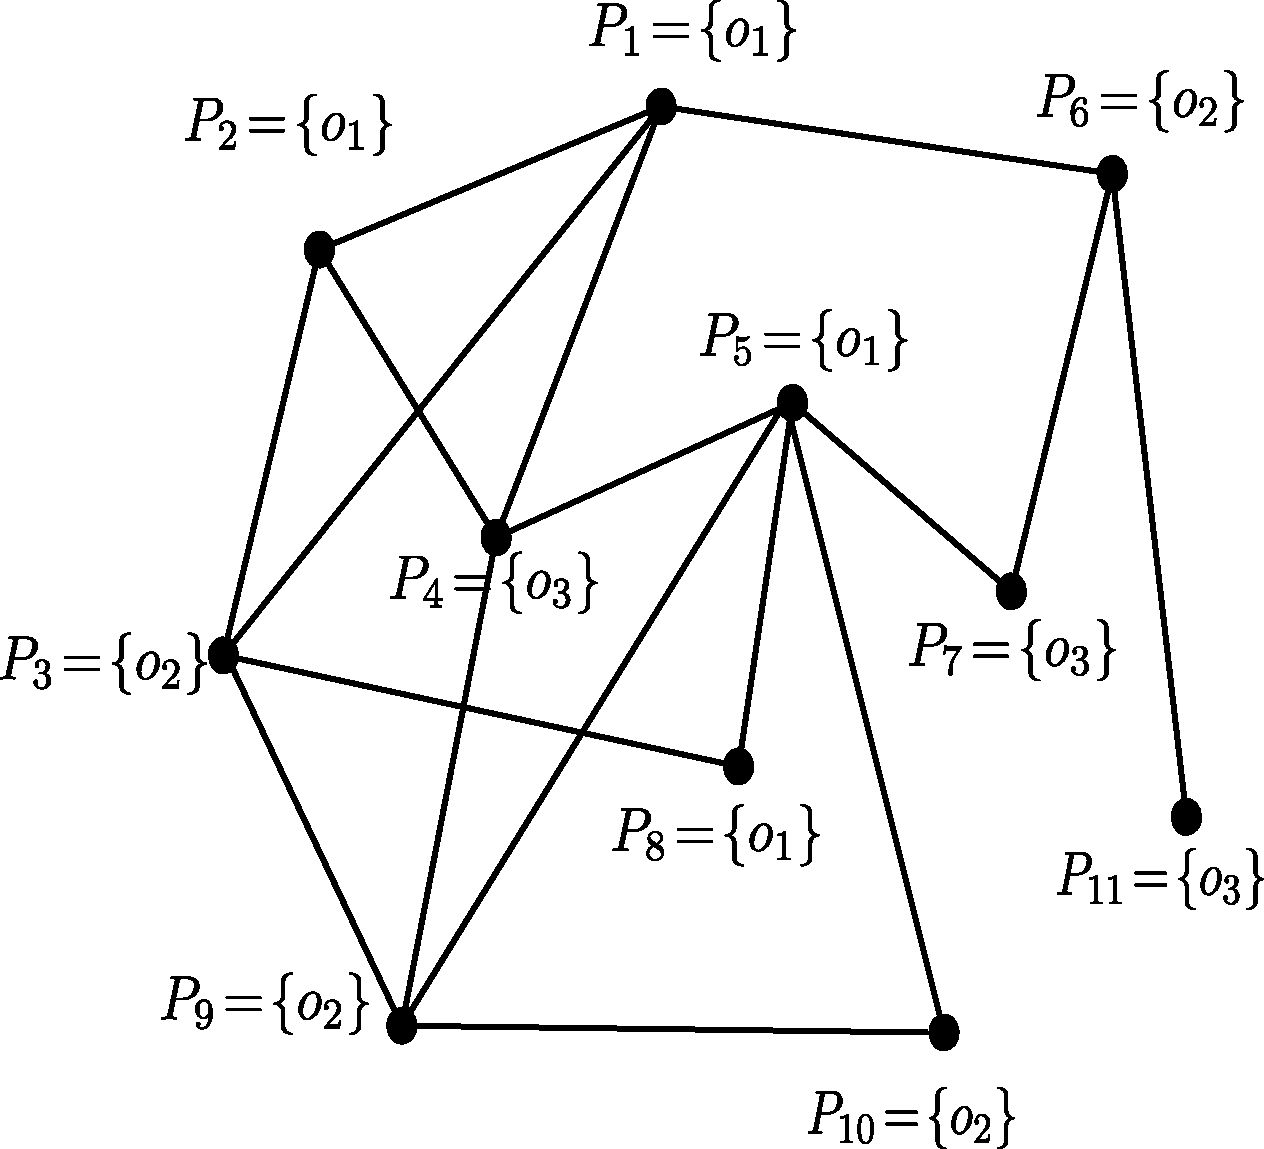
\includegraphics[totalheight=.22\textheight,
width=.4\textwidth,viewport=-50 0 800 750]{example} \hspace{0.4in}
\end{center}
\vspace{-0.3cm}\caption{CSR game with $n=11$ players and $O=\{o_1,o_2,o_3\}$ resources. We have $C_1(P)=0+1+1=2, C_8(P)=0+1+2=3$ and $r_1(P)=1, r_8(P)=1$.}
\label{fig:example-model}
\end{figure}
\vspace{-0.3cm}
\begin{remark}
If some resource $o$ is missing in an allocation profile $P$, we define the cost of each player for that specific resource to be large, e.g., $d_{\mathcal{G}}(i, \sigma_i(P, o)) = D + 1, \forall i \in [n]$. Therefore, for $n \ge |O|$, this incentivizes at least one of the players to allocate the missing resources in the network. In the case where $n < |O|$, all the players will allocate different resources and the game becomes trivial, hence we can simply assume that $n \ge |O|$.
\end{remark}

\begin{remark}\label{rem:varying-cache}
Actually all the proofs in this paper can be carried over to games with varying capacities by constructing a new network which transfers games with different cache sizes to one with unit size caches \cite{etesami2014pure,gopalakrishnan2012cache}.
\end{remark}

\begin{remark}\label{rem:cost-to-radius}
Given two allocation profiles $P$ and $\tilde{P}$ which only differ in the $i$th coordinate, using \eqref{eq:CSR-cost-formulation} and the definition of the radius, one can easily see that $C_i(P)-C_i(\tilde{P})=r_i(\tilde{P})-r_i(P)$. This establishes an equivalence between decrease in cost and increase in radius for player $i$, when the actions of the other players are fixed.
\end{remark}

It has been shown in \cite{gopalakrishnan2012cache} that the CSR game has an associated ordinal potential function, and hence, it has at least one pure Nash equilibrium. More precisely

\smallskip
\begin{theorem}\label{thm:existence-NE}
The CSR game admits an ordinal potential function, and hence, a pure-strategy Nash equilibrium.
\end{theorem}

Although Theorem \ref{thm:existence-NE} proves the existence of NE, however, in general it can only gurantee an exponential number of iterations for finding such equilibrium points ($\mathcal{O}(|O|^n)$). Therefore, the main challenge here is to find an efficient way to arrive at an equilibrium which we will address in the remaining of this paper.
